\documentclass{jsarticle}
\oddsidemargin=-0.8cm
\topmargin=-2cm
\baselineskip=13pt
\textheight=55\baselineskip
\marginparsep=0.5in
\marginparwidth=0.5in
\textwidth=52zw
\usepackage{ascmac}
\usepackage{url}
\usepackage[dvips]{graphicx}
\usepackage{amsmath}
\usepackage{amssymb}
\usepackage{multicol}
\usepackage{bm}
\usepackage{enumerate}
\usepackage{listings}
\usepackage{fancybox}
\usepackage{framed}
\usepackage{subfigure}
\usepackage{ccaption}
\usepackage{color}
\makeatletter
\lstset{% 
language={C}, 
frame=trbl,% 
basicstyle={\small},% 
identifierstyle={\small},% 
commentstyle={\small\ttfamily},% 
keywordstyle={\small\bfseries},% 
ndkeywordstyle={\small},% 
stringstyle={\small\ttfamily}, 
tabsize=2,
breaklines=true, 
frame=none,
columns=[l]{fullflexible},% 
numbers=left,% 
xrightmargin=0zw,% 
xleftmargin=3zw,% 
numberstyle={\scriptsize},% 
stepnumber=1, 
numbersep=1zw,% 
backgroundcolor={\color[gray]{.90}},
} 
\makeatother

\newenvironment{problems}
{
  \renewcommand\labelenumi{\doublebox{\arabic{enumi}}}
  \begin{enumerate}
}{
  \end{enumerate}
  \renewcommand\labelenumi{\arabic{enumi}.}
}

\pagestyle{empty}	

\begin{document}
\title{基礎気象学講義 補足プリント} % ここは毎回同じ
\author{第9回} %authorの代わりに第何回かを入れる
\date{気象力学の重要な応用:数値予報} %内容を記載する
\maketitle

\section{はじめに}
現代の天気予報が、スーパーコンピュータによる計算を行って出されているということは、義務教育の教科書にまで掲載されており、もはや人口に膾炙しているといえよう。
だが、どういった計算が行われているかという詳細については気象力学等を始めとした専門性ゆえにブラックボックスと化している。
本講義では、このコンピュータによる予報―数値予報―の概要について、気象庁発行の数値予報解説資料\footnote{\url{https://www.jma.go.jp/jma/kishou/books/nwpkaisetu/nwpkaisetu.html}}や数値予報60年誌\footnote{\url{https://www.jma.go.jp/jma/kishou/know/whitep/1-3-2-1.html}}を基礎に解説する。次いで、数値予報モデルの計算結果について、予報資料を概観する。最後に、実際の現象を数値的に解いて数値予報を体験する。

本プリントは、この内「数値予報体験」の部分について記したものである。

\section{数値予報体験}
現実の数値予報は、多くの観測データと大規模な格子から、スーパーコンピュータを用いて計算しなければとても求められない程のものであるが、簡単な計算であれば家庭などにあるコンピュータでも可能である。

この場では、数値予報より簡単な、具体的な観測結果を用いない仮想的な例での問題を設定し、数値的に予報を行うとはどういうことか体験してみよう。

\subsection{問題設定}
単位質量の質点がコリオリ力の影響下において運動しているケースを考える。この他に単位質点にかかる力はなく、初速は$(u,v)=(u_0,v_0)$により与えられるとする。この時、この質点の運動方程式は
\[
\left\{
\begin{array}{l}
\frac{du}{dt}=fv \\
\frac{dv}{dt}=-fu
\end{array}
\right.
\]

により与えられる。この運動は慣性振動を表しており、解析的な解により運動を考察できる\footnote{余力があったら、実際に計算してみると数値予報結果と比較しやすい。誤差解析にも有用である。}が、ここではこれを題材に数値予報を行ってみる。

\subsection{数値解法}
数値的に微分方程式を解くためには、微分をうまく近似・離散化し、時間的発展を表した漸化式に直した上で、四則演算により計算できる形に直さねばならない。

\subsubsection{Euler法}
微分の定義を考えれば、
\[
u'(t)\approx \frac{u(t+\Delta t)-u(t)}{\Delta t}
\]
である。これを\textbf{前進差分近似}といい、$\Delta t$に比例した誤差を含む近似である\footnote{誤差については、$u(t+\Delta t)$をテイラー展開して計算すれば良い。}。

今、$u(n\Delta t)=u_n$などと、時間$n\Delta t$における物理量を$n\in \mathbb{N}_0$を添え字として記すことにする。慣性振動の方程式は
\[
\left\{
\begin{array}{l}
u_{n+1}=u_n+fv_n\Delta t \\
v_{n+1}=v_n-fu_n\Delta t
\end{array}
\right.
\]
と与えられる。定数並びに$\Delta t$を適切に定め、この漸化式に従って予報したい時間の$u,v$並びに$x,y$を求めれば\footnote{位置についても同様の近似を行い、$x_{n+1}=x_n+u_n \Delta t$という式で計算すれば良い。}、それが数値予報の結果を示す。

この近似方法による時間発展方程式の解法を\textbf{Euler法}と呼ぶ。

\subsubsection{Leap-Frog法}
Euler法とは別の近似手法を導入してみよう。

$u(t\pm \Delta t)$をテイラー展開し、その差を取ることで次の式(\textbf{中央差分近似})が得られる。

\[
u'(t)\approx \frac{u(t+\Delta t)-u(t-\Delta t)}{2 \Delta t}
\]

これを慣性運動の方程式に代入すれば、
\[
\left\{
\begin{array}{l}
u_{n+1}=u_{n-1}+2fv_n\Delta t \\
v_{n+1}=v_{n-1}-2fu_n\Delta t
\end{array}
\right.
\]
である。位置についても同様に
\[
x_{n+1}=x_{n-1}+2u_n\Delta t
\]
が成立する。

添字が1の場合に限りEuler法を適用し、その後はこの一連の方法(Leap-Frog法)を用いて計算すれば、誤差は$O(\Delta t^2)$となる。

\subsection{結果の整理}
ここでは、Euler法についてのみ述べるので、Leap-frog法での計算は自身で行ってみてほしい。

$f=4.18\times 10^{-5}$(日本付近での値)、$u_0=v_0=0.1$m/s、$\Delta t=600$s、初期は原点という条件下で、Euler法で導出した式に従って2日分の位置を計算した\footnote{表計算ツールでも計算可能であるし、プログラムなどを書いても構わない。}。
結果を図\ref{Euler}に示す。

\begin{figure}[ht]
\centering
\includegraphics[width=0.6\linewidth,clip,keepaspectratio]{Euler.eps}
\caption{Euler法による慣性振動の計算結果。点の間はスプライン補間し、実線にて記した。}\label{Euler}
\end{figure}

慣性振動という名のとおり、これは振動あるいは円運動にならなければおかしいが、実際には少しずれている。これは、計算誤差による影響であり、エネルギーが増大しているのも同様と考えられよう。


\section{一般に公開されているモデル}
 数値予報モデルは各国の気象機関のみが用いているわけではなく、教育・研究その他に向けて公開されている。日本語情報のある2例を紹介しておく。

\begin{itemize}
\item 気象庁のモデルは、無条件公開というわけではないが、「数値予報研究開発プラットフォーム」\footnote{\url{http://pfi.kishou.go.jp/}}にて利用申請をすることで研究目的での利用が可能である。
\item 一方、より広く教育等に向けて使えるモデルとしては、地球流体電脳倶楽部\footnote{\url{https://www.gfd-dennou.org/}}のものがよく知られている。このサイトでは、最新のデータなども取得することができ、教育・研究活動に向く。
\end{itemize}


\end{document}

